% **************************************************************************************************
% ** SPSC Report and Thesis Template
% **************************************************************************************************
%
% ***** Authors *****
% Daniel Arnitz, Paul Meissner, Stefan Petrik
% Signal Processing and Speech Communication Laboratory (SPSC)
% Graz University of Technology (TU Graz), Austria
%
% ***** Changelog *****
% 0.1   2010-01-25   extracted from report template by Daniel Arnitz (not ready yet)
% 0.2   2010-02-08   added thesis titlepage and modified layout (not ready yet)
% 0.3   2010-02-18   added TUG logo and statutory declaration
% 0.4   2010-02-18   moved the information fields below \input{./base/packages} (encoding...)
% 0.5   2010-03-02   added \ShortTitle to fix problems with long thesis titles
%                    added \ThesisType (makes the template suitable for MSc, BSc, PhD, ... Thesis)
%
% ***** Todo *****
% - Introduction/Usage
% **************************************************************************************************

% **************************************************************************************************
% basic setup
\newcommand{\DocumentType}{report} % "thesis" / "report"
\newcommand{\DocumentLanguage}{de} % "en" / "de"
\newcommand{\Twosided}{} % "twoside" / ""


% **************************************************************************************************
% template setup -- do not change these unless you know what you are doing!
\input{./base/packages}
\input{./base/layout_\DocumentType}
\input{./base/macros}
\graphicspath{{./drawings/}{./plots/}{./images/}}
% **************************************************************************************************
% ATTENTION: Make sure that makeindex is set to -s "./base/index.sty"
% **************************************************************************************************

% uncomment to get watermarks:
% \usepackage[first,bottom,light,draft]{draftcopy}
% \draftcopyName{ENTWURF}{160}


% **************************************************************************************************
% information fields

% general
\newcommand{\DocumentTitle}{Computational Intelligence UE}
\newcommand{\DocumentSubtitle}{Homework 1: Linear Regression}
\newcommand{\ShortTitle}{CI Homework 1} % used in headers (keep short!)
\newcommand{\DocumentAuthor}{Thomas Ebner, Raphael Hoheneder, Stefan N\"ohmer}
\newcommand{\DocumentDate}{Graz, \today}
%    for thesis only (will be ignored for reports)
\newcommand{\ThesisType}{Master's Thesis}
\newcommand{\Organizations}{Signal Processing and Speech Communications Laboratory \\ Graz University of Technology \\[1cm] on behalf of \\ Some Company} % SPSC \\ TUG \\[1cm] on behalf of \\ A Nice Company
\newcommand{\Advisors}{Dipl.-Ing. Dr. Assoc.Prof. Klaus Witrisal \\ Dipl.-Ing. Paul Meissner} % Advisor 1 \\ Advisor 2 \\ ...
\newcommand{\Supervisors}{Univ.-Prof. Dipl.-Ing. Dr.techn. Gernot Kubin}

% revision number
\newcommand{\RevPrefix}{alpha~}
\newcommand{\RevLarge}{1}
\newcommand{\RevSmall}{1}

% confidential?
\newcommand{\ConfidNote}{confidential}% {"confidential", "eyes only", ...}

% short command for vectors
\newcommand{\vect}[1]{\mathbf{#1}}


\begin{document}
% **************************************************************************************************
% titlepage
\input{./base/titlepage_\DocumentType}

% statutory declaration for theses
\ifthenelse{\equal{\DocumentType}{thesis}}{\input{./base/declaration}}{}


% **************************************************************************************************
% **************************************************************************************************
% user-defined part

\chapter{Homework: Linear Regression}
\section{Linear Regression with Non-Linear Basis-Functions}
\subsection{Task 1.1.1: Polynomial Basis Functions}

\subsubsection{Aufgabenstellung:}


Es sollen die Gewichtungsfaktoren f�r Polynome vom 0ten Grad bis zum 18ten Grad gefunden werden, dazu sind die 60 gegebenen X- und Y-Trainingswerte zu verwenden.


Danach sind die Trainingspunkte, die Target-Funktion(y\_target) und die ``Lern-funktionen'' zu Auszugeben.


Die Basisfunktionen als Funktion von X ausgeben.

Ausgeben des ``Mean Squared Error'' (MSE) f�r die Trainings- und Test- werte.


\subsubsection{Plots \& Diskussion:}
\begin{figure}[hp!]
\begin{center}
 \includegraphics[width=0.99\textwidth]{./figures/1_1_1_unscaled_learn_fct}
 \caption[Unskalierte Lernfunktionen]{Unskalierte Lernfunktionen}
\label{fig:unscaled_learn_fct}
\end{center}
\end{figure}


\begin{figure}[hp!]
\begin{center}
 \includegraphics[width=1\textwidth]{./figures/1_1_1_scal_learn_fct}
 \caption[Skalierte Lernfunktionen]{Skalierte Lernfunktionen}
\label{fig:scal_learn_fct}
\end{center}
\end{figure}

In Abbildung \ref{fig:unscaled_learn_fct} sehen wir die Lernfunktionen.
In Abb. \ref{fig:unscaled_learn_fct} reisen die Werte f�r Polynome h�heren Grades am Ende des ``Plots'' sehr stark aus.
 Das Bild wird somit in Y-Richtung gequetscht wird, in Abb. \ref{fig:scal_learn_fct} das ganze noch einmal skaliert um mehr zu erkennen.

\begin{figure}[hp!]
\begin{center}
 \includegraphics[width=1\textwidth]{./figures/1_1_1_base_fct}
 \caption[Basisfunktionen als Funktion von X]{Basisfunktionen als Funktion von X}
\label{fig:base_fct}
\end{center}
\end{figure}



Bei Funktionen mit h�heren Polynomen ist die Funktion zwar sehr gut eingepasst an die Trainingspunkte, neigt aber zu starkem �berschwingen.
Das sog. ``Overfitting'' tritt hier auf.
\clearpage

\begin{figure}[hp!]
\begin{center}
 \includegraphics[width=1\textwidth]{./figures/1_1_1_MSE}
 \caption[Mean Square Error]{Mean Square Error f�r Trainings- und Test-Werte}
\label{fig:MSE}
\end{center}
\end{figure}

Wie man in Abb. \ref{fig:MSE} sehen kann ist bereits bei einer Funktion mit Grad 8 der Fehler sehr gering,bei Grad 8 ist  
Aufwand und Leistung am Besten. Es ist die Funktion nur f�r die Trainings-Werte 
perfekt angepasst allerdings wird durch das ``OverFitting'' f�r alle anderen Werte der Fehler wieder gr��er.
\subsection{Task 1.1.2: Radial Basis Functions}


\subsubsection{Aufgabenstellung:}
Nun ist die Basisfunktion eine Gau\ss{} 'sche Glockenkurve die mit $\phi_k(x) = exp(-(x-\mu_k)^2 /\sigma^2 )$ gegeben ist.
Wobei $d=2:18$, $\sigma$ $= 2/d$ und $\mu =d$ schritten zwischen -1 und 1 entspricht.
Es sind wieder  die Trainingspunkte, die Target-Funktion (y\_target) und die gelernten Funktionen auszugeben.
Die Basisfunktion ist mit $d=6,12$ und $18$ als Funktion von x zu plotten.
Ausgeben des ``Mean Squared Error'' (MSE) für die Trainings- und Testwerte.



\subsubsection{Plots \& Diskussion}


\begin{figure}[h!]
\begin{center}
 \includegraphics[width=1\textwidth]{./figures/RBF_learn}
 \caption[Trainingspunkte, Target-Funktion und Lernfunktionen]{Trainingspunkte, Target-Funktion und Lernfunktionen}
\label{fig:RBF_learn}
\end{center}
\end{figure}



Wie man in Abb. \ref{fig:RBF_learn} sehen kann ist das ``Ausbrechen'' bei der Radial-Funktion am Ende bei weitem nicht so ausgeprägt!

\begin{figure}[h!]

\begin{center}
 \includegraphics[width=0.75\textwidth]{./figures/RBF_6}
 \caption[Basisfunktionen als Funktion von X (d=6)]{Basisfunktionen als Funktion von X mit einem $d=6$}
\label{fig:RBF_6}
\end{center}
\end{figure}

\begin{figure}[h!]
\begin{center}
 \includegraphics[width=0.75\textwidth]{./figures/RBF_12}
 \caption[Basisfunktionen als Funktion von X, d=12]{Basisfunktionen als Funktion von X mit einem $d=12$}
\label{fig:RBF_12}
\end{center}
\end{figure}


\begin{figure}[h!]
\begin{center}
 \includegraphics[width=0.75\textwidth]{./figures/RBF_18}
 \caption[Basisfunktionen als Funktion von X, d=18]{Basisfunktionen als Funktion von X mit einem $d=18$}
\label{fig:RBF_18}
\end{center}
\end{figure}

Man kann erkennen, dass auch hier bei höherer Ordnung die Steilheit zunimmt. Gau\ss{}'sch-Funktionen neigen allerdings nicht zum ``Ausbrechen'',
da sie wenn sie Richtung unendlich gehen keinen ``Schaden'' anrichten, da sie wieder zu ihrem Nullpunkt zurückkehren.
Was sich auch in Abb. \ref{fig:RBF_MSE} zeigt, da hier der MSE der Testwerte bei hohem Grad nicht so stark ansteigt wie in Bsp.1.1.1.
 

\begin{figure}[h!]
\begin{center}

 \includegraphics[width=0.8\textwidth]{./figures/RBF_MSE}
 \caption[MSE]{MSE des Trainingsset und des Testsets.}
\label{fig:RBF_MSE}
\end{center}
\end{figure}
\clearpage

\subsection{Task 1.1.3: Local Linear Models}

In diesem Beispiel ist die Designmatrix X doppelt so groß wie vorher. War sie in Task 1.1.2 noch $(60 \times d)$ groß, ist sie jetzt $(60 \times 2d)$. Neben der G


\subsection{Task 1.1.4: Regularized Polynomial Regression}

%nöhmes stuff:

\paragraph{Regularized Regression Grundlagen}

Folgende Fehlerfunktion soll minimal werden:

$$ E(\vect{w}) = \frac{1}{N} \sum_{i=1}^N(y_i - \sum_{k=1}^d \Phi_k(x_i) w_k)^2 + \alpha^2 \sum_{k=1}^d w_k^2 $$

Zuerst müssen die indizierten Variablen in Vektoren umgeschrieben werden:

$$ \vect{x} = \begin{bmatrix} x_1 \\ x_2 \\ \vdots \\ x_N \end{bmatrix}, \; \vect{y} = \begin{bmatrix} y_1 \\ y_2 \\ \vdots \\ y_N \end{bmatrix}, \; \vect{w} = \begin{bmatrix} w_1 \\ w_2 \\ \vdots \\ w_d \end{bmatrix}, \; \vect{\Phi}(\vect{x}) = \begin{bmatrix} \Phi_1(\vect{x}) \\ \Phi_2(\vect{x}) \\ \vdots \\ \Phi_d(\vect{x}) \end{bmatrix} $$

wobei $ \vect{x} \in M(N \times 1), \; \vect{y} \in M(N \times 1), \; \vect{w} \in M(d \times 1), \; \vect{\Phi}(\vect{x}) \in M(d \times 1) $.

Nun können die Summen in Matrixform umgeschrieben werden (von innen nach aussen):

$$ \sum_{k=1}^d \Phi_k w_k = \vect{\Phi}^T \cdot \vect{w}, \; \text{da} \begin{bmatrix} \Phi_1 && \Phi_2 && \hdots && \Phi_d \end{bmatrix} \cdot \begin{bmatrix} w_1 \\ w_2 \\ \vdots \\ w_d \end{bmatrix} = \Phi_1 w_1 + \Phi_2 w_2 + \hdots + \Phi_d w_d \; \text{(Skalar)} $$

$$ \alpha^2 \sum_{k=1}^d w_k^2 = \alpha^2 \cdot \vect{w}^T \cdot \vect{w}, \; \text{aus dem selben Grund wie oben (ebenfalls Skalar)} $$

Mit der gleichen Regel kann man auch die äußere Summe zusammenfassen:

$$ \sum_{i=1}^N (y_i - \sum_{k=1}^{d} \Phi_k(x_i) w_k)^2 = (\vect{y} - \vect{\Phi}(\vect{x})^T \vect{w})^T (\vect{y} - \vect{\Phi}(\vect{x})^T \vect{w}), \; \text{dim} = (N \times d) $$

Also ergibt sich die gesamte Fehlerfunktion als:

$$ E(\vect{w}) = \frac{1}{N} (\vect{y} - \vect{\Phi}(\vect{x})^T \vect{w})^T (\vect{y} - \vect{\Phi}(\vect{x})^T \vect{w}) + \alpha^2 \vect{w}^T \vect{w} \; \text{(Skalar)} $$

Die Matrix $ \vect{\Phi}(\vect{x})^T $ wird im folgenden als Designmatrix $ \vect{X} $ abgekürzt und hat folgende Form:

$$ \vect{X} = \vect{\Phi}(\vect{x})^T = \begin{bmatrix} \Phi_1(x_1) && \Phi_2(x_1) && \hdots && \Phi_d(x_1) \\  \Phi_1(x_2) && \Phi_2(x_2) && \hdots && \Phi_d(x_2) \\ \vdots && \ddots \\ \Phi_1(x_N) && \Phi_2(x_N) && \hdots && \Phi_d(x_N) \end{bmatrix} $$

Ihre Dimension ist also $ \vect{X} \in M(N \times d) $.

Um nun den Fehler zu minimieren, muss die Fehlerfunktion abgeleitet werden:

$$ \frac{\partial E(\vect{w})}{\partial \vect{w}} = \frac{\partial}{\partial \vect{w}} \frac{1}{N} (\vect{y} - \vect{X} \vect{w})^T (\vect{y} - \vect{X} \vect{w}) + \alpha^2 \vect{w}^T \vect{w} $$

Mit $ \frac{\partial \vect{w}^T \vect{w}}{\partial \vect{w}} = 2 \vect{w}^T $ (Matrix-Cookbook, (10)) ergibt sich (innere Ableitung nicht vergessen!):

$$ \frac{\partial E(\vect{w})}{\partial \vect{w}} = - \frac{2}{N} (\vect{y} - \vect{X} \vect{w})^T \vect{X} + 2 \alpha^2 \vect{w}^T $$

Um das Minimum zu finden, wird diese Ableitung jetzt 0 gesetzt und auf $\vect{w}$ umgeformt:

$$ - \frac{2}{N} (\vect{y} - \vect{X} \vect{w})^T \vect{X} + 2 \alpha^2 \vect{w}^T = 0 $$
$$ \frac{2}{N} (\vect{y} - \vect{X} \vect{w})^T \vect{X} = 2 \alpha^2 \vect{w}^T $$
$$ (\vect{y} - \vect{X} \vect{w})^T \vect{X} = N \alpha^2 \vect{w}^T $$
$$ (\vect{y}^T - \vect{w}^T \vect{X}^T) \vect{X} = N \alpha^2 \vect{w}^T $$
$$ \vect{y}^T \vect{X} - \vect{w}^T \vect{X}^T \vect{X} = N \alpha^2 \vect{w}^T $$
$$ \vect{w}^T \vect{X}^T \vect{X} + N \alpha^2 \vect{w}^T = \vect{y}^T \vect{X} $$
$$ \vect{w}^T \vect{X}^T \vect{X} + \vect{w}^T N \alpha^2 = \vect{y}^T \vect{X} $$
$$ \vect{w}^T (\vect{X}^T \vect{X} + N \alpha^2 \vect{I}) = \vect{y}^T \vect{X} $$
$$ \vect{w}^T = \vect{y}^T \vect{X} (\vect{X}^T \vect{X} + N \alpha^2 \vect{I})^{-1} $$
$$ \vect{w} = (\vect{X}^T \vect{X} + N \alpha^2 \vect{I})^{-1} \vect{X}^T \vect{y} $$
%endlich!!! :)


%tom stuff:



\paragraph{Polynomial Basis Functions}


Wie in der Abbildung \ref{fig:poly_mse} zu sehen ist, ergibt sich ein minima des MSE der Testdaten
bei $\alpha = 0.00015167$. Wie in der Abbildug \ref{fig:poly_learned} zu sehen ist, bewirkt ein höherer Wert von
$\alpha$ ein Abflachen der Lernkurve. Bei kleineren Werten von $\alpha$ ist die Kurve weniger abgeflacht und
folgt mehr den Trainigsdaten. Ein kleinerer Wert von $\alpha$ hat jedoch den entscheidenden Nachteil, dass ausserhalb
des Bereichs der Trainingsdaten(auf der x-Achse), die Lernkurve sehr stark nach oben bzw. unten wegknickt.
$\alpha$ vergrößert bei größeren Gewichten die Fehlerfunktion $E(x)$ und wirkt somit dem entgegen.

Der mean squared error korrelliert sehr gut dem Mittelwert der absoluten Gewichte. Für Größere Werte von $\alpha$
ergibt sich verbessert sich der MSE bei den Trainings- und Testdaten. Wird jedoch $\alpha$ zu groß gewählt, so steigt
der MSE wieder.


  \begin{center}
	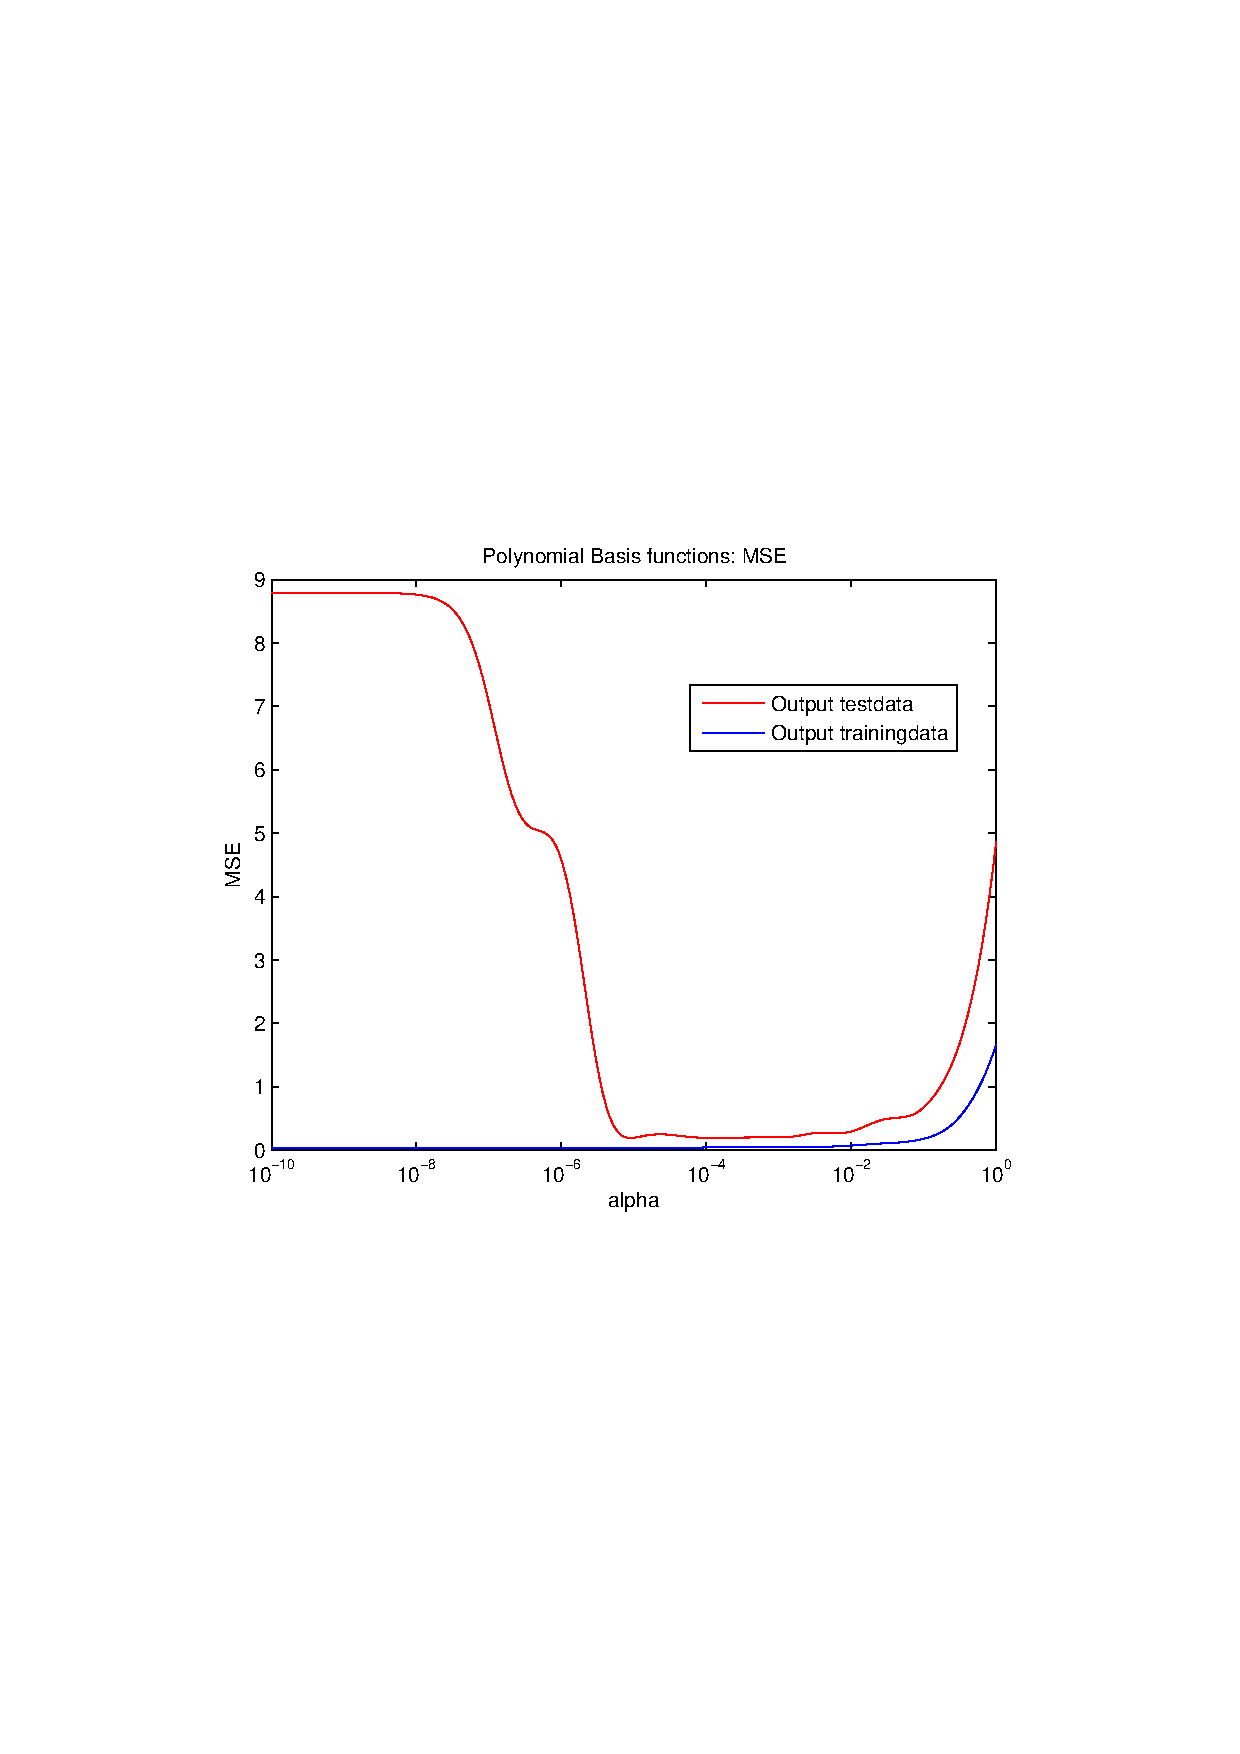
\includegraphics[width=15cm]{figures/114/poly_mse.png}
	\captionof{figure}{Polynomial Basis Functions: Mean squared error, Minimum bei $\alpha = 0.00015167$}
	\label{fig:poly_mse}
  \end{center}

  \begin{center}
	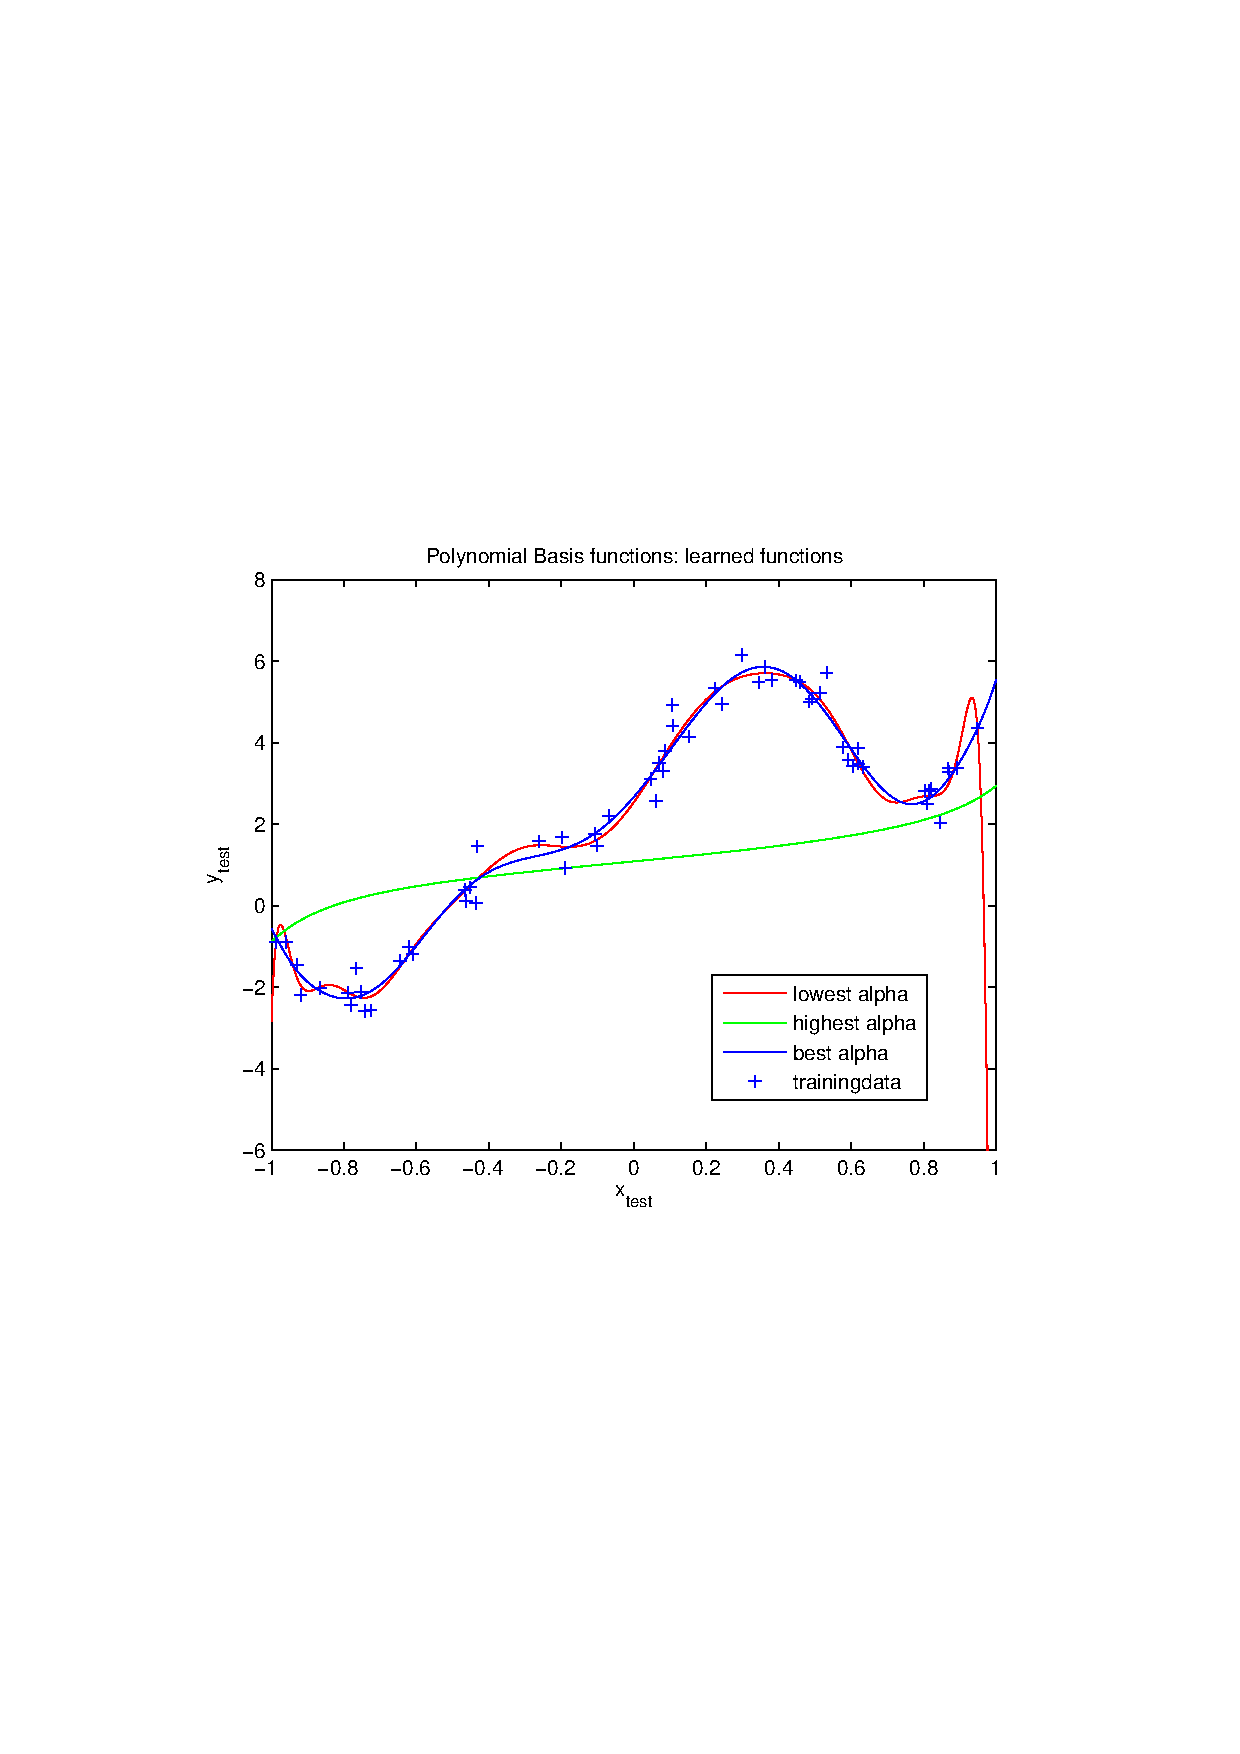
\includegraphics[width=15cm]{figures/114/poly_learned.png}
	\captionof{figure}{Polynomial Basis Functions: learned output function}
	\label{fig:poly_learned}
  \end{center}

  \begin{center}
	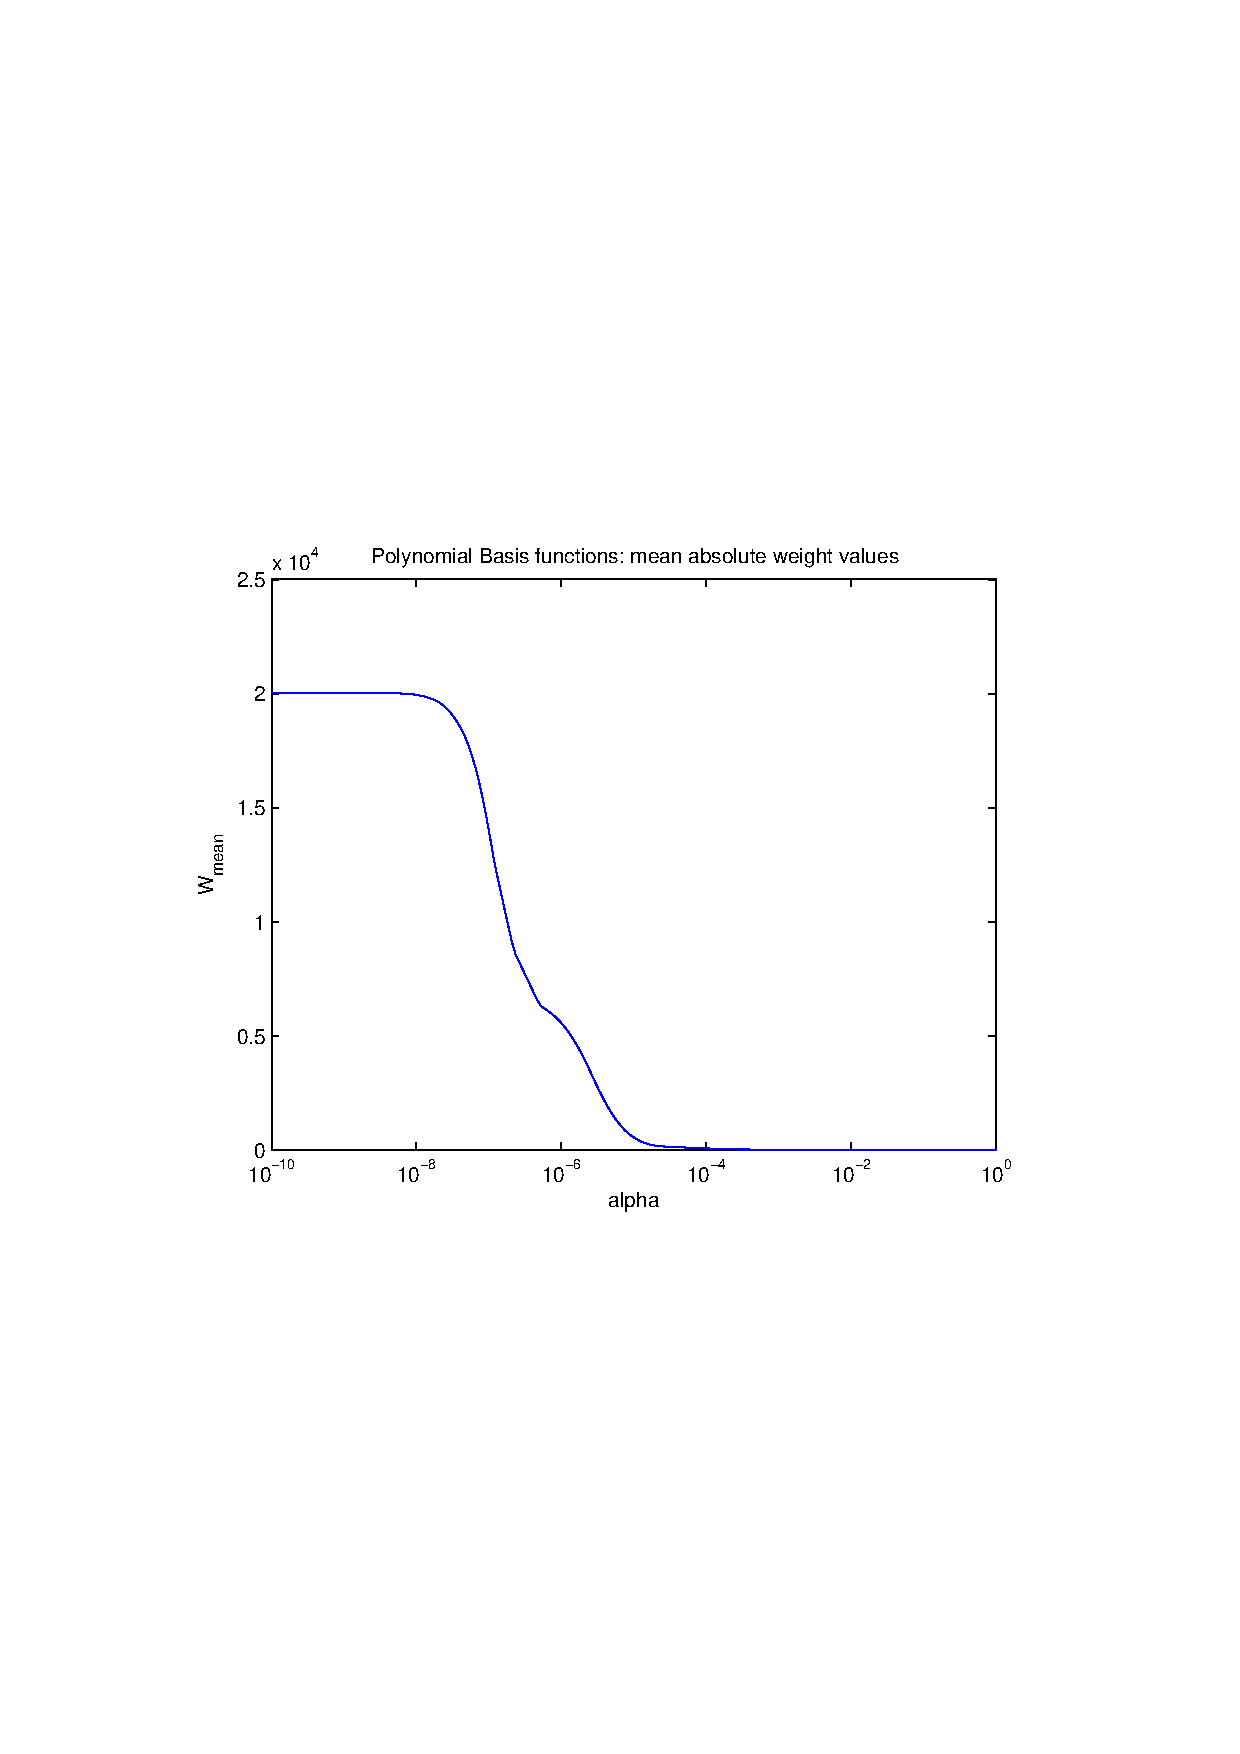
\includegraphics[width=15cm]{figures/114/poly_meanweight.png}
	\captionof{figure}{Polynomial Basis Functions: mean absolute weight over $\alpha$}
	\label{fig:poly_meanweight}
  \end{center}


\paragraph{Radial Basis Functions}

Wie in der Abbildung \ref{fig:radial_mse} zu sehen ist, ergibt sich ein minima des MSE der Testdaten
bei $\alpha = 0.021964$. Wie in der Abbildug \ref{fig:radial_learned} zu sehen ist, bewirkt ein höherer Wert von
$\alpha$ keine wesentliche Verbesserung, so wie Beispielsweise bei den polynomialen Basisfunktionen.

Der mean squared error korrelliert bei den Radialen Basisfunktionen gar nicht mit dem MSE der Testdaten, was
auch nocheinmal zum Ausdruck bringt, dass der Trick mit dem $\alpha$ fast zu keiner Verbesserung führt.
Eine mögliche Begründung dafür wäre, dass bei den Radialen Basisfunktionen auch ohne $\alpha$ die Lernkurve
an den Rändern der Testdaten nur wenig wegknickt.


  \begin{center}
	\includegraphics[width=15cm]{figures/114/radial_mse.png}
	\captionof{figure}{Radial Basis Functions: Mean squared error, Minimum bei $\alpha = 0.021964$}
	\label{fig:radial_mse}
  \end{center}

  \begin{center}
	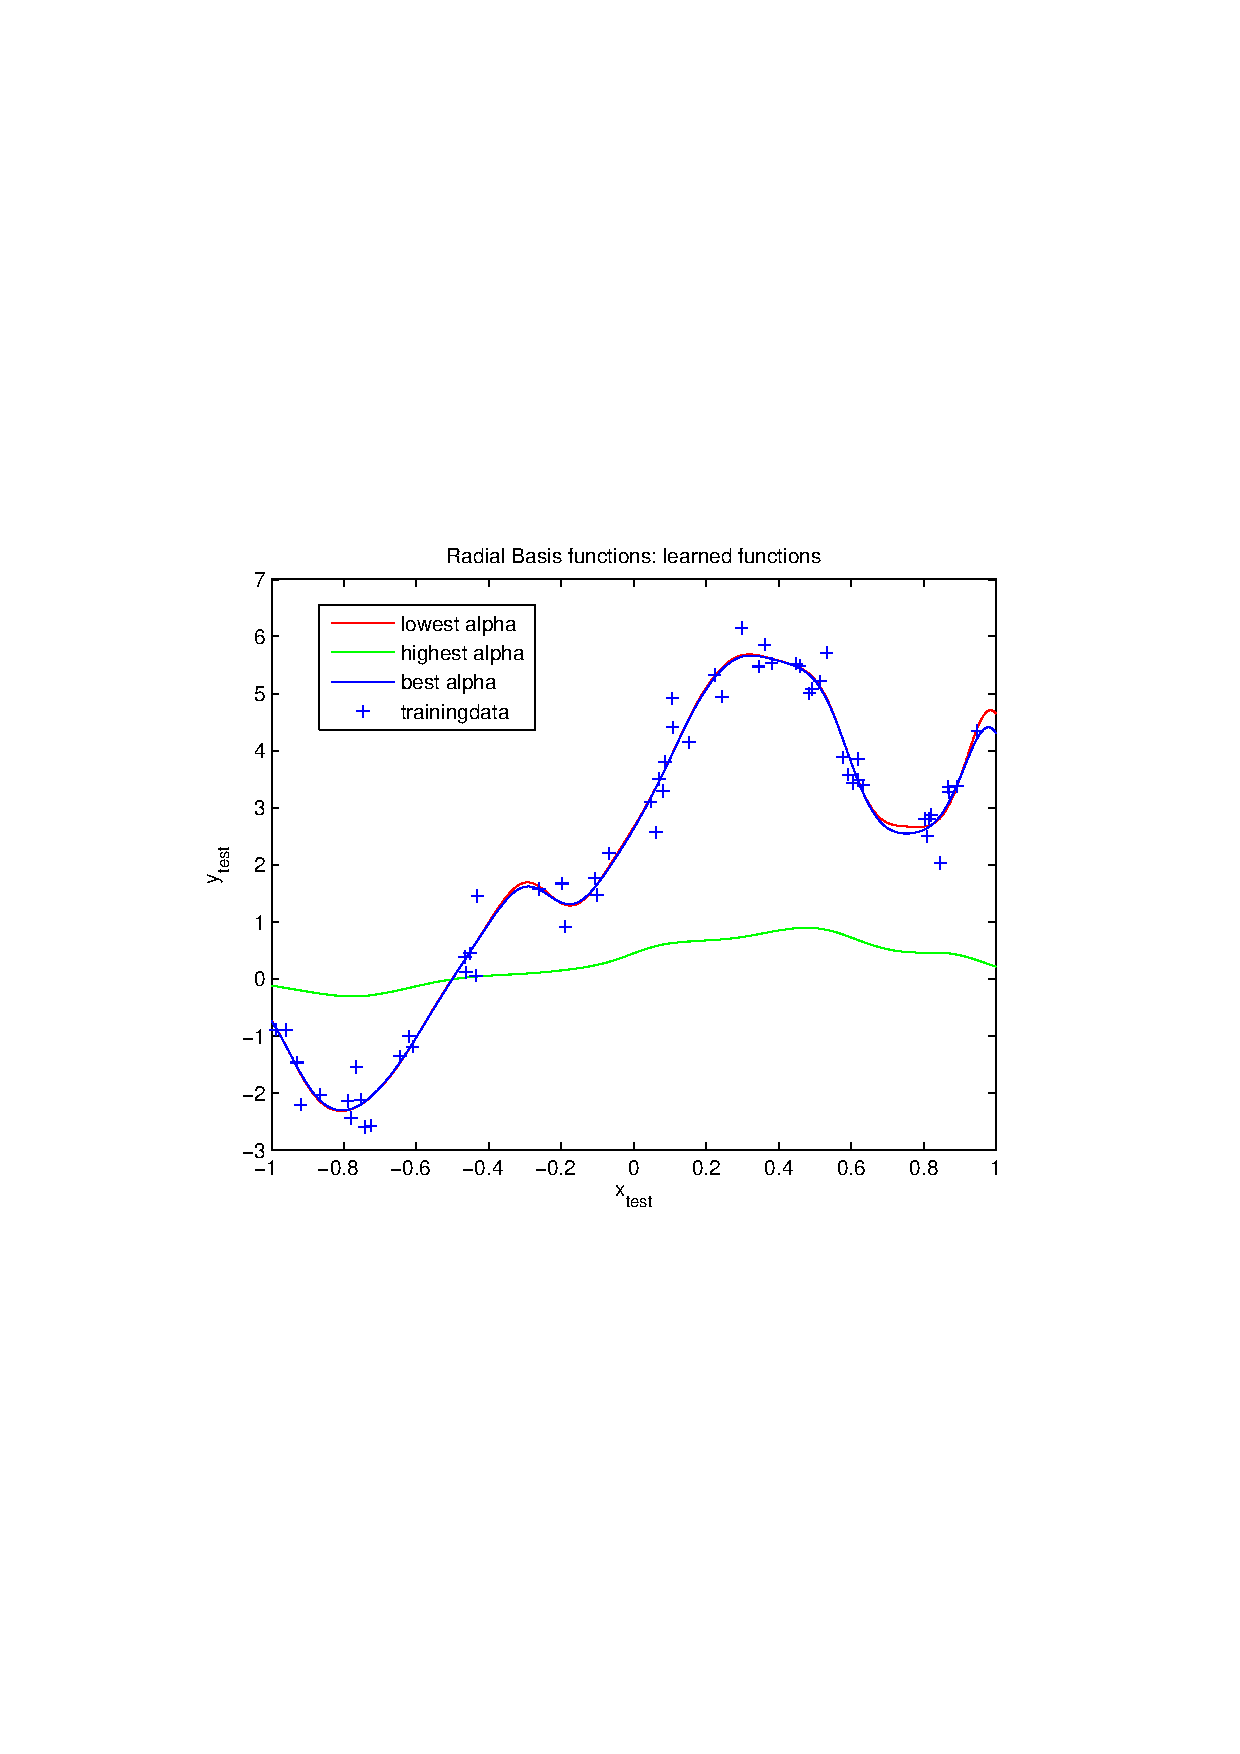
\includegraphics[width=15cm]{figures/114/radial_learned.png}
	\captionof{figure}{Radial Basis Functions: learned output function}
	\label{fig:radial_learned}
  \end{center}

  \begin{center}
	\includegraphics[width=15cm]{figures/114/radial_meanweight.png}
	\captionof{figure}{Radial Basis Functions: mean absolute weight over $\alpha$}
	\label{fig:radial_meanweight}
  \end{center}



\paragraph{Local linear models}


Wie in der Abbildung \ref{fig:local_mse} zu sehen ist, ergibt sich ein minima des MSE der Testdaten
bei $\alpha = 0.034891$. Wie in der Abbildug \ref{fig:local_learned} zu sehen ist, bewirkt ein höherer Wert von
$\alpha$ ein Abflachen der Lernkurve. Bei kleineren Werten von $\alpha$ ist die Kurve deutlich weniger abgeflacht und
folgt mehr den Trainigsdaten. Ein kleinerer Wert von $\alpha$ hat jedoch den entscheidenden Nachteil, dass ausserhalb
des Bereichs der Trainingsdaten(auf der x-Achse) und sogar zwischen größeren Abständen
zwischen den Trainingsdaten, die Lernkurve sehr stark nach oben bzw. unten wegknickt. Die Lernkurve für kleinere $\alpha$
ist eigentlich fast unbrauchbar.
$\alpha$ vergrößert bei größeren Gewichten die Fehlerfunktion $E(x)$ und wirkt somit dem entgegen.

Der mean squared error korrelliert sehr gut dem Mittelwert der absoluten Gewichte. Für Größere Werte von $\alpha$
ergibt sich verbessert sich der MSE bei den Trainings- und Testdaten. Wird jedoch $\alpha$ zu groß gewählt, so steigt
der MSE wieder.


  \begin{center}
	\includegraphics[width=15cm]{figures/114/local_mse.png}
	\captionof{figure}{Local linear models: Mean squared error, Minimum bei $\alpha = 0.034891$}
	\label{fig:local_mse}
  \end{center}

  \begin{center}
	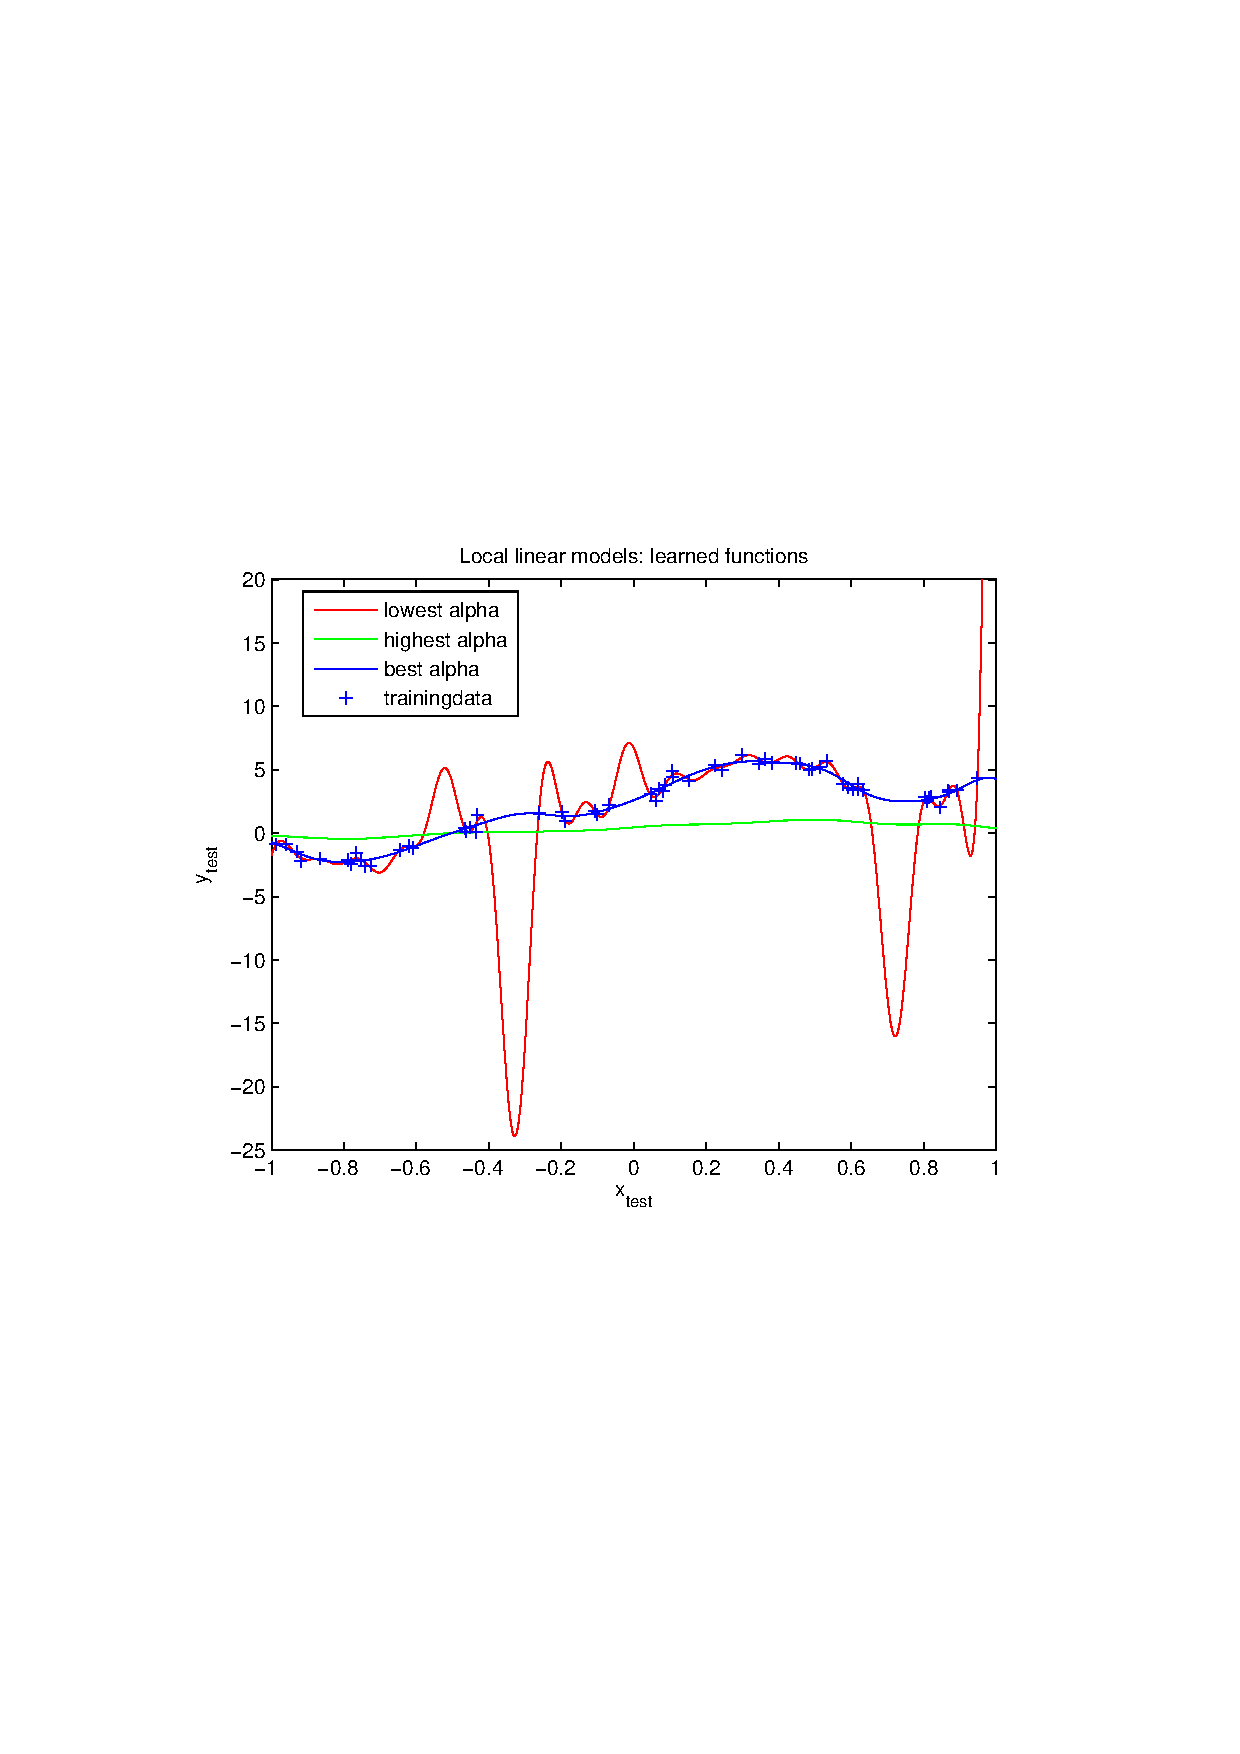
\includegraphics[width=15cm]{figures/114/local_learned.png}
	\captionof{figure}{Local linear models: learned output function}
	\label{fig:local_learned}
  \end{center}

  \begin{center}
	\includegraphics[width=15cm]{figures/114/local_meanweight.png}
	\captionof{figure}{Local linear models: mean absolute weight over $\alpha$}
	\label{fig:local_meanweight}
  \end{center}


\paragraph{Vergleich}

Bei den angegebenen Trainings- und Testdaten konnte mithilfe der Polynimialen Basisfunktionen das Beste
Ergebnis erzielt werden. Dabei Betrug der MSE ca. 0.189, hingegen bei den beiden anderen Verfahren ca. 0.2.
Bei Local linear Model führte der Term mit $\alpha$ zu einer deutlichen Verbesserung der Ergebnise, wobei
man bei den Radialen Basisfunktionen, den $\alpha$ - Term auch weglassen könnte ohne deutliche schlechtere
Ergebnise zu erzielen.


% **************************************************************************************************
% **************************************************************************************************

%\appendix
%\bibliographystyle{/.base/ieeetran}
%\bibliography{_bibliography}

% place all floats and create label on last page
\FloatBarrier\label{end-of-document}
\end{document}

